\chapter{Benchmarks}

\citet{KoTr02a,KoTr02b} carefully benchmarked the spectral-element
simulations of global seismic waves against normal-mode seismograms.
Version 4.0 of \texttt{SPECFEM3D\_GLOBE} has been benchmarked again
following the same procedure.

In this appendix we present two tests: a `long-period' (periods longer
than 17~s) simulation of a shallow event in isotropic PREM \citep{DzAn81}
without the ocean layer, without attenuation but including the effects
of self-gravitation (in the Cowling approximation) (Figures \ref{fig:Vanuatu-with-Vertical}
and \ref{fig:Vanuatu-with-Transverse}), and a `short-period' (periods
longer than 9~s) simulation of a deep event in transversely isotropic
PREM without the ocean layer and including the effects of self-gravitation
and attenuation (Figures \ref{fig:Bolivia-with-Vertical}, \ref{fig:Bolivia-with-Transverse}
and \ref{fig:Bolivia-PKP}).

%
\begin{figure}[ht]
\noindent \begin{centering}
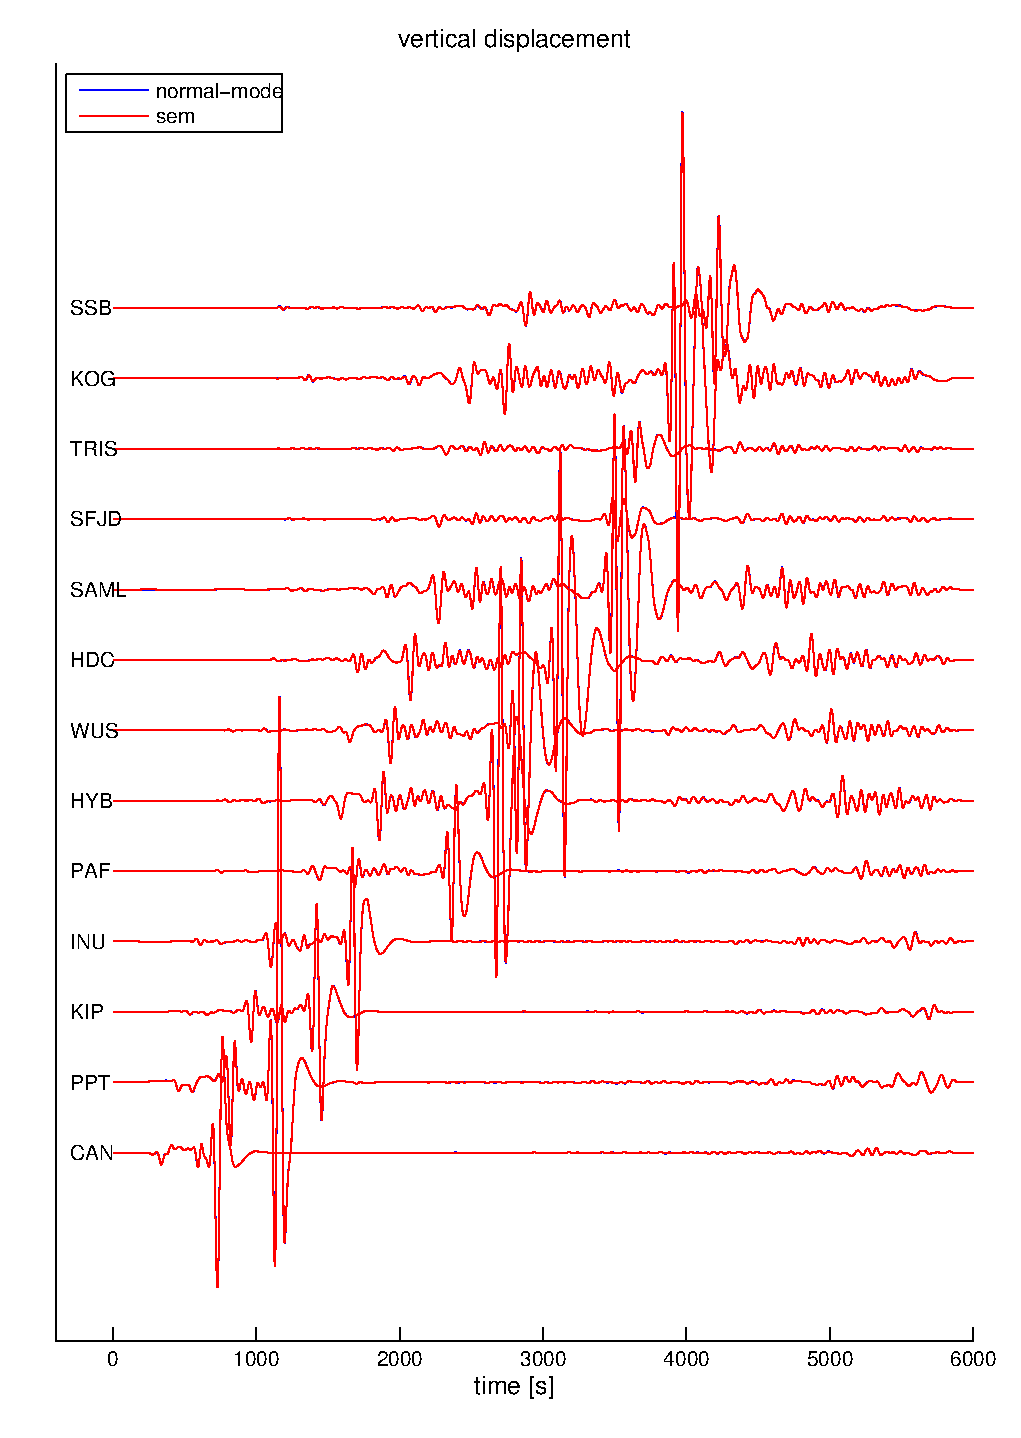
\includegraphics[scale=0.75]{figures/vanuatu_vertical.pdf}
\caption{Normal-mode (blue) and SEM (red)
vertical displacements in isotropic PREM considering the effects of
self-gravitation but not attenuation for 13 stations at increasing
distance from the 1999 November 26th Vanuatu event located at 15~km
depth. The SEM computation is accurate for periods longer than 17~s.
The seismograms have been filtered between 50~s and 500~s. The station
names are indicated on the left. }
\label{fig:Vanuatu-with-Vertical}

\par\end{centering}
\end{figure}
%
\begin{figure}[ht]
\noindent \begin{centering}
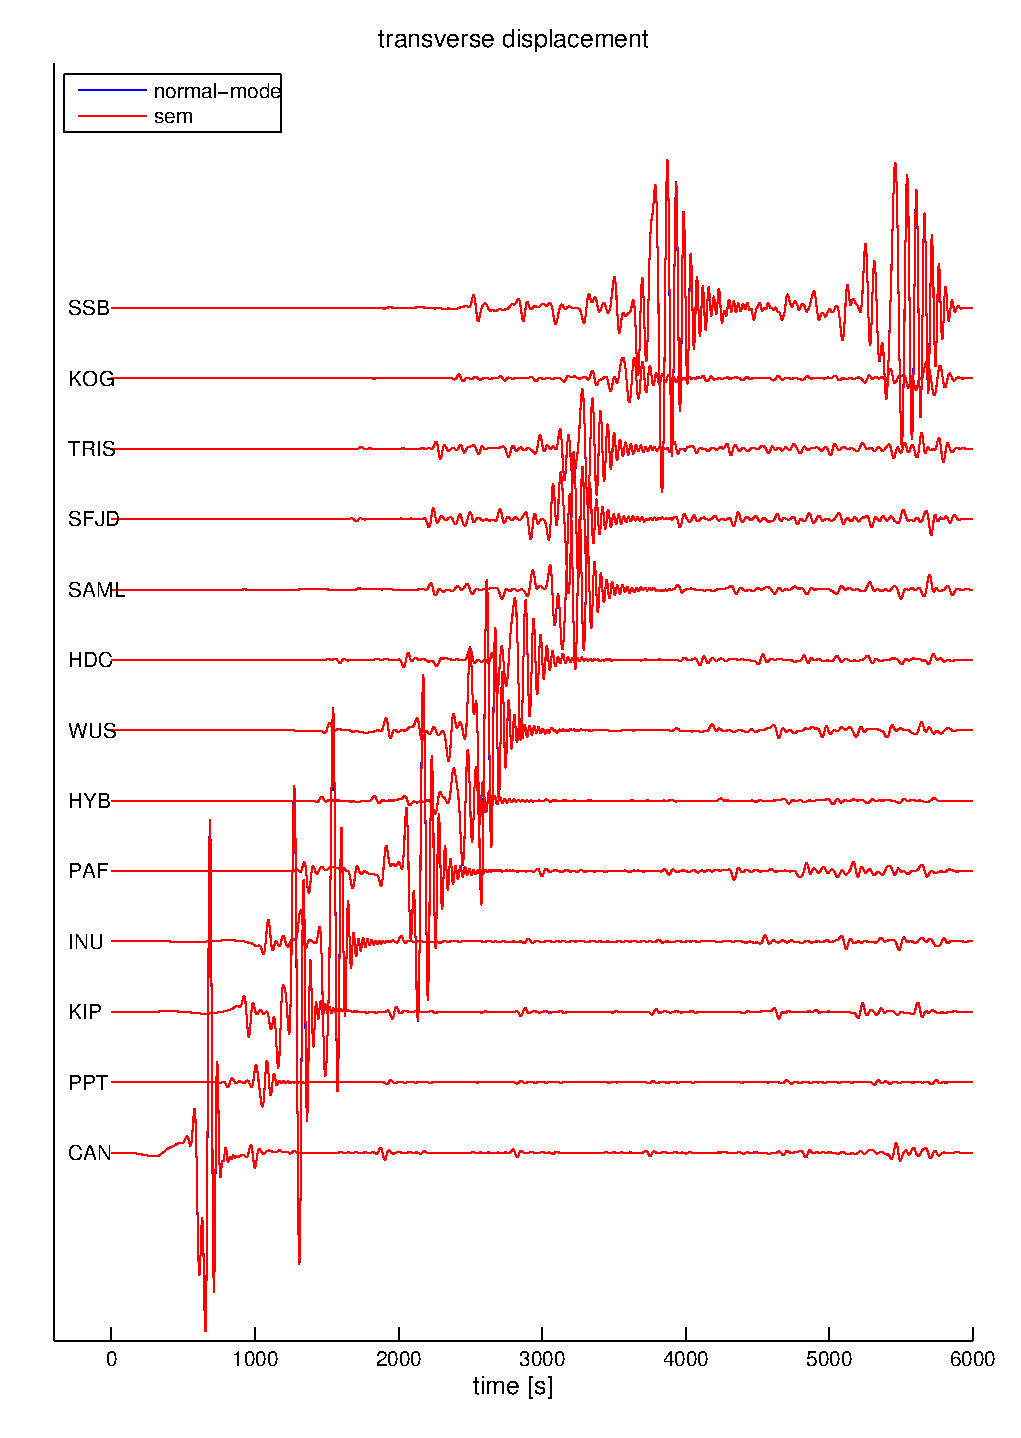
\includegraphics[scale=0.75]{figures/vanuatu_trans.pdf}
\caption{Same as in Figure \ref{fig:Vanuatu-with-Vertical}
for the transverse displacements.}
\label{fig:Vanuatu-with-Transverse}

\par\end{centering}
\end{figure}
%
\begin{figure}[ht]
\noindent \begin{centering}
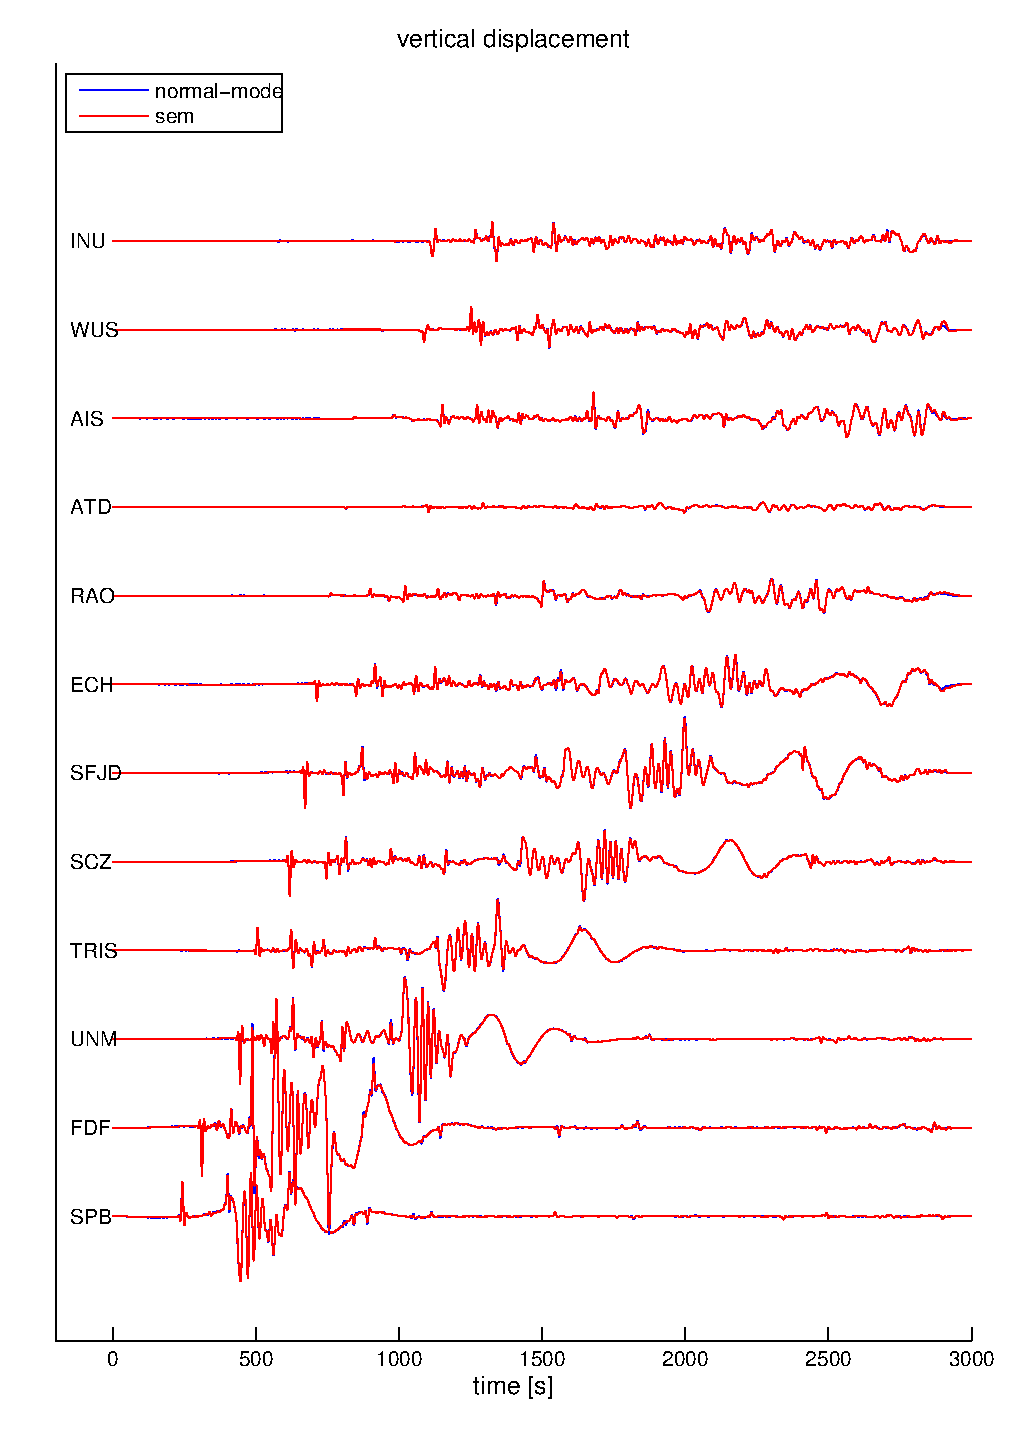
\includegraphics[scale=0.75]{figures/bolivia_vertical.pdf}
\caption{Normal-mode (blue) and SEM (red)
vertical displacements in transversely isotropic PREM considering
the effects of self-gravitation and attenuation for 12 stations at
increasing distance from the 1994 June 9th Bolivia event located at
647~km depth. The SEM computation is accurate for periods longer
than 9~s. The seismograms have been filtered between 10~s and 500~s.
The station names are indicated on the left.}
\label{fig:Bolivia-with-Vertical}

\par\end{centering}
\end{figure}
%
\begin{figure}[ht]
\noindent \begin{centering}
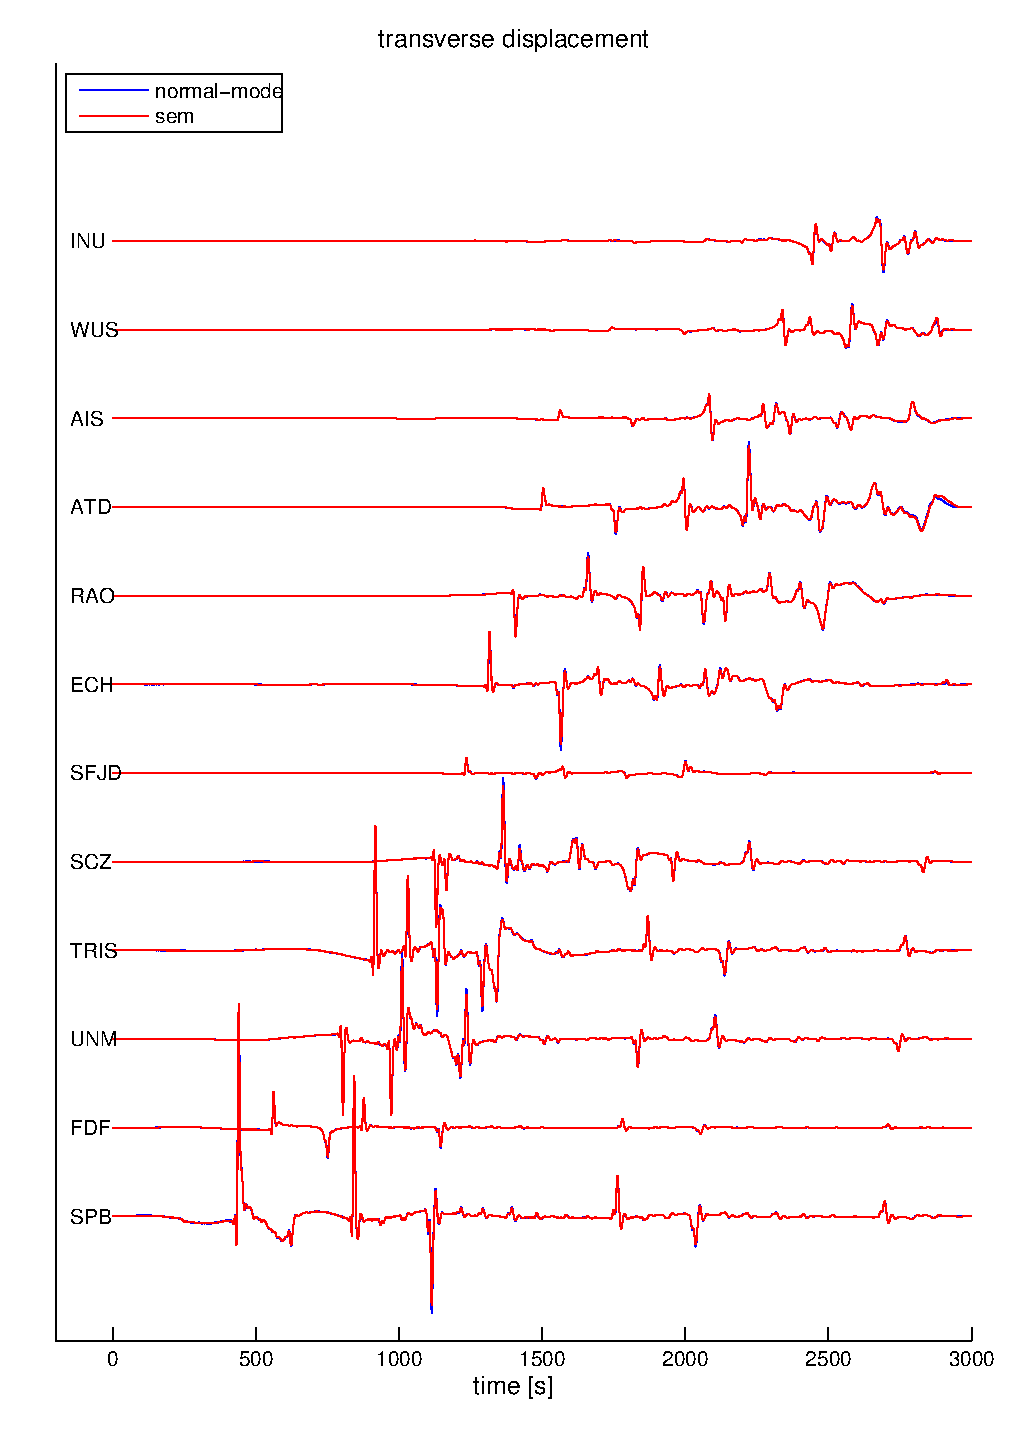
\includegraphics[scale=0.75]{figures/bolivia_trans.pdf}
\caption{Same as in Figure \ref{fig:Bolivia-with-Vertical}
for the transverse displacements.}
\label{fig:Bolivia-with-Transverse}

\par\end{centering}
\end{figure}


%
\begin{figure}[ht]
\noindent \begin{centering}
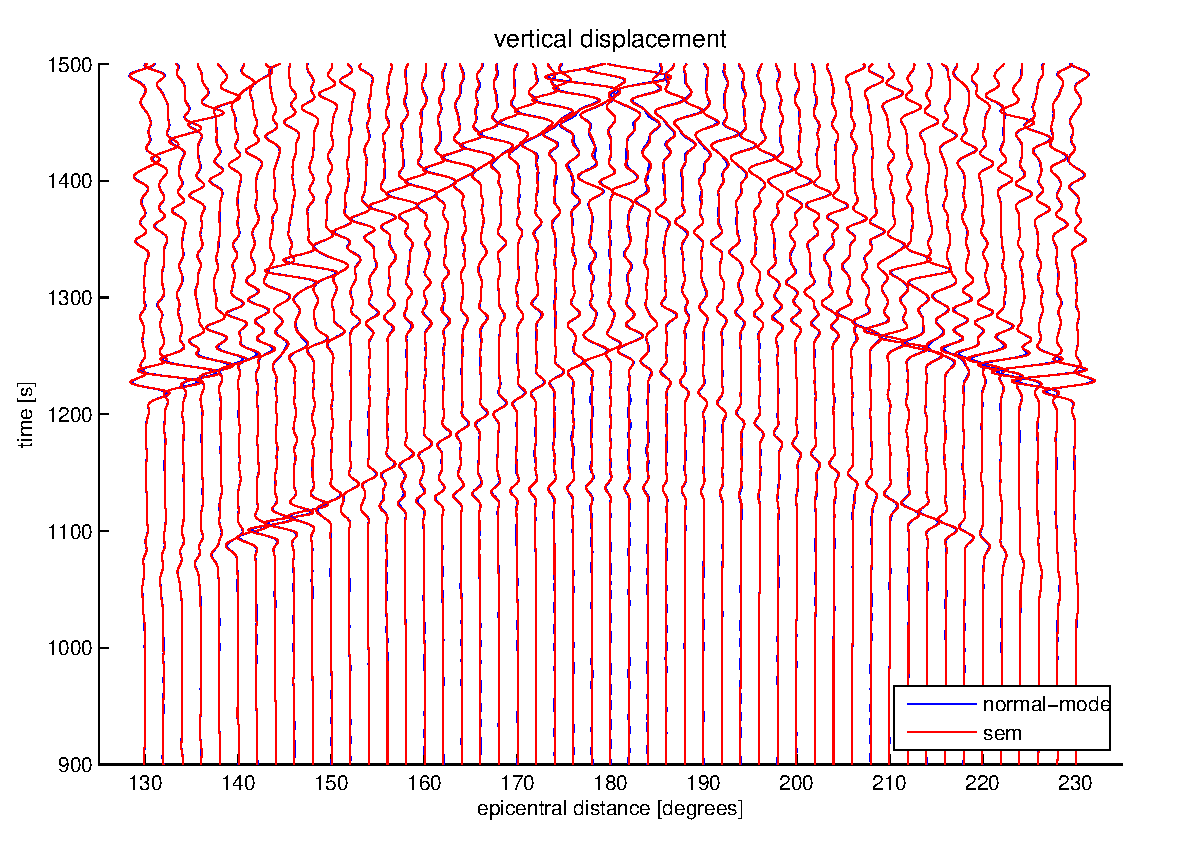
\includegraphics[scale=0.75]{figures/PKPdf_all_15s500s.pdf}
\caption{Seismograms recorded between 130 degrees and
230 degrees, showing in particular the good agreement for core phases
such as PKP. This figure is similar to Figure 24 of \citet{KoTr02a}.
The results have been filtered between 15~s and 500~s.}
\label{fig:Bolivia-PKP}

\par\end{centering}
\end{figure}


The normal-mode synthetics are calculated with the code \texttt{QmXD}
using mode catalogs with a shortest period of 8~s generated by the
code \texttt{OBANI}. No free-air, tilt, or gravitational potential
corrections were applied \citep{DaTr98}. We also turned off the effect
of the oceans in \texttt{QmXD}.

The normal-mode and SEM displacement seismograms are first calculated
for a step source-time function, i.e., setting the parameter \texttt{half}
\texttt{duration} in the \texttt{CMTSOLUTION} file to zero for the
SEM simulations. Both sets of seismograms are subsequently convolved
with a triangular source-time function using the processing script
\texttt{UTILS/seis\_}~\\
\texttt{process/process\_syn.pl}. They are also band-pass filtered
and the horizontal components are rotated to the radial and transverse
directions (with the script \texttt{UTILS/seis\_process/rotate.pl}).

The match between the normal-mode and SEM seismograms is quite remarkable
for the experiment with attenuation, considering the very different
implementations of attenuation in the two computations (e.g., frequency
domain versus time domain, constant Q versus absorption bands).

Further tests can be found in the \texttt{EXAMPLES} directory. It
contains the normal-mode and SEM seismograms, and the parameters (\texttt{STATIONS},
\texttt{CMTSOLUTION} and \texttt{Par\_file}) for the SEM simulations.

Important remark: when comparing SEM results to normal mode results, one needs to
convert source and receiver coordinates from geographic to geocentric coordinates,
because on the equator the geographic and
geocentric latitude are identical but not elsewhere. Even for
spherically-symmetric simulations one must perform this conversion
because the source and receiver locations provided by globalCMT.org and
IRIS involve geographic coordinates.




